\documentclass[11pt]{article}
\usepackage{geometry}
\geometry{margin=1in}
\usepackage{amssymb}
\usepackage{enumitem}
\usepackage{parskip}
\usepackage{xcolor}
\usepackage{tikz}
\definecolor{benblue}{HTML}{1769AA}
\definecolor{benorange}{HTML}{C2410C}
\definecolor{bengreen}{HTML}{38761D}

\newcommand{\drawbox}[1]{%
  \par\vspace{4pt}\noindent
  \fbox{\rule{0pt}{#1}\rule{\dimexpr\linewidth-2\fboxsep-2\fboxrule}{0pt}}%
  \par\vspace{6pt}}

\newcommand{\task}[1]{\par\medskip\noindent\textbf{\color{benblue}#1}\par\nopagebreak}

\title{\vspace{-1.5cm}\textbf{Why every triangle adds up to 180}\\[-2pt]
  \large Where proof begins}
\author{}
\date{}

\begin{document}
\maketitle
\vspace{-1.2cm}

\noindent\textbf{The big idea.} Tear the three corners off any triangle and they
snap together into a straight line. A straight line is $180^\circ$, so the three
angles add to $180$. The real question: \emph{why must this happen for every
triangle, even ones nobody has drawn yet?}

\section*{Activity: tear three different triangles}
\begin{enumerate}[leftmargin=*]
  \item Draw three triangles that look nothing alike: a long skinny one, a fat
        one, a pointy one.
  \item Shade the three corners of each so you can tell them apart.
  \item \textbf{Tear} (do not cut neatly) the three corners off each triangle.
  \item Slide the three torn corners together, points touching, and see what they
        make.
\end{enumerate}
\task{Draw your three triangles here, then tape the reassembled corners below them:}
\drawbox{4.5cm}

\task{Every time, the three corners make a \underline{\hspace{3cm}}, which is
\underline{\hspace{2cm}} degrees.}

\section*{The proof: a parallel line through the top}
Take any triangle $ABC$. Through the top vertex $A$, draw a line \emph{parallel to
the bottom side $BC$}. Three angles sit along that straight line at $A$:
$x$, the apex angle $A$, and $y$.

\begin{center}
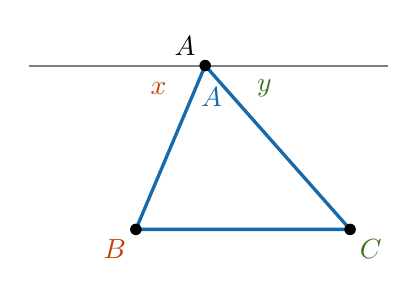
\begin{tikzpicture}[scale=1.6, line join=round]
  \coordinate (A) at (0.55,1.3);
  \coordinate (B) at (0,0);
  \coordinate (C) at (1.7,0);
  % parallel helper line through A
  \draw[gray, thick] (-0.85,1.3) -- (2.0,1.3);
  % triangle
  \draw[benblue, very thick] (A) -- (B) -- (C) -- cycle;
  % vertices
  \foreach \p in {A,B,C} \fill (\p) circle (1.3pt);
  \node[above left] at (A) {$A$};
  \node[below left,benorange] at (B) {$B$};
  \node[below right,bengreen] at (C) {$C$};
  % the three angles along the line at A
  \node[benorange] at (0.18,1.12) {$x$};
  \node[benblue]   at (0.6,1.05)  {$A$};
  \node[bengreen]  at (1.02,1.12) {$y$};
\end{tikzpicture}
\end{center}

Because $x$, $A$, $y$ lie along a straight line, $\;x + A + y = 180.$ The ``Z''
(alternate-angles) rule says $x = B$ and $y = C$, because of the parallel lines.

\task{Substitute $x=B$ and $y=C$ into $x + A + y = 180$. What do you get? Why does
this prove it for \emph{every} triangle and not just yours?}
\drawbox{2.6cm}

\section*{Push further}
\begin{enumerate}[leftmargin=*]
  \item \textbf{Four sides.} Split any quadrilateral into two triangles with one
        diagonal. Its four angles add to \underline{\hspace{2cm}} degrees.
  \item \textbf{Many sides.} An $n$-sided polygon splits into $n-2$ triangles, so
        its angles add to $(n-2)\times 180$. Check it on a pentagon
        ($5$ sides $\Rightarrow$ \underline{\hspace{2cm}}).
  \item \textbf{Competition gem: the five-pointed star.} Draw a five-pointed star
        in one stroke. \textbf{What do the five point-angles add up to?} (Hint:
        each point is the tip of a little triangle; chase the angles with the
        $180$ rule.)
        \drawbox{3.5cm}
  \item \textbf{True or false?} Guess first, then check.
        \begin{itemize}
          \item The three angles of a triangle always add to $180$. \hfill T \quad / \quad F
          \item A very pointy triangle adds to \emph{more} than $180$. \hfill T \quad / \quad F
          \item The five points of \emph{any} star add to $180$. \hfill T \quad / \quad F
        \end{itemize}
\end{enumerate}

\end{document}
